\section{Das Perceptron}
Zu Beginn steht das Perceptron. Es wird hier wie in Abbildung \ref{fig:04_perceptron} veranschaulicht.
Es besteht aus der Summe mehrerer gewichteter Eingabewerte wie auch einem Bias, welcher
die Schwelle einer Aktivierung verschiebt. Die Gewichte werden mit $w_i$, die Eingabewerte mit $x_i$ bezeichnet.
Diese Summe, im folgenden als $net$ bezeichnet, wird in eine Aktivierungsfunktion,
hier eine Sigmoide, gegeben. Der resultierende Wert wird als $z$ bezeichnet. Der Bias hat den festen Wert $-1$,
er wird wiederum über ein Gewicht $w_0$ trainiert.

\begin{figure}[h!]
    \begin{center}
        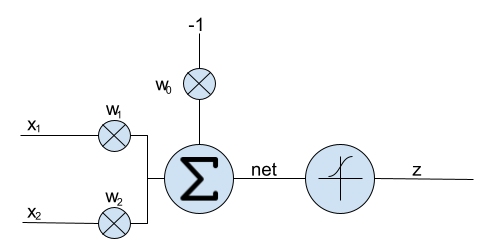
\includegraphics[width=0.6\linewidth]{../common/01_perceptron/00_resources/00_perceptron.png}
    \end{center}
    \caption{Das Perceptron}
    \label{fig:04_perceptron}
\end{figure}

\subsection{Lernverfahren}

\subsection{Das Problem mit XOR und nichtlinearen Funktionen}